\documentclass[7pt]{article}
\usepackage{amsmath}
\usepackage{graphicx}
\usepackage{caption}
\usepackage[landscape]{geometry}
\usepackage{multicol}
\usepackage{amssymb}
\usepackage{geometry}
 \geometry{
 a4paper,
 total={285mm,185mm},
 left=10mm,
 top=10mm,
 }
\setcounter{section}{4}
\setlength\columnseprule{0.5pt}
\setlength{\parindent}{0pt}
\graphicspath{ {images/} }


\begin{document}
\begin{multicols*}{3}

\section{Mechanische Wellen}
\subsection{Wellenfunktion}
\begin{equation*}
  \xi = \xi(x,t)
\end{equation*}
x = Raumkoordinate\newline
t = Zeit\newline

\paragraph{Wellentypen:}
\begin{enumerate}
  \item Seilwellen: $\xi(x,t)$ beschreibt transversale Auslenkung des Seils
  \item Federwellen: $\xi(x,t)$ beschreibt transversale oder logitudinale Verformung der Feder
  \item Gaswellen: $\xi(x,t)$ beschreibt den Druck des Gase 
\end{enumerate}

\paragraph{Vereinfachung - Weglassen der Dispersion}\mbox{}\\
Normalerweis ver{\"a}ndert sich die Form des Wellenberges mit der Zeit (=Dispersion). Wir werden dies allerdings weglassen und den Wellenberg als stabile Form betrachten.

Zudem nehmen wir die Welle zur Zeit t=0 an. Daraus folgt:
\begin{equation*}
  \xi(x, t=0) = f(x)  
\end{equation*}
\paragraph{Welle nach links:}
\begin{equation*}
\xi = f(x-vt) 
\end{equation*}
\paragraph{Welle nach rechts:}
\begin{equation*}
\xi = f(x+vt) 
\end{equation*}
\begin{center}
	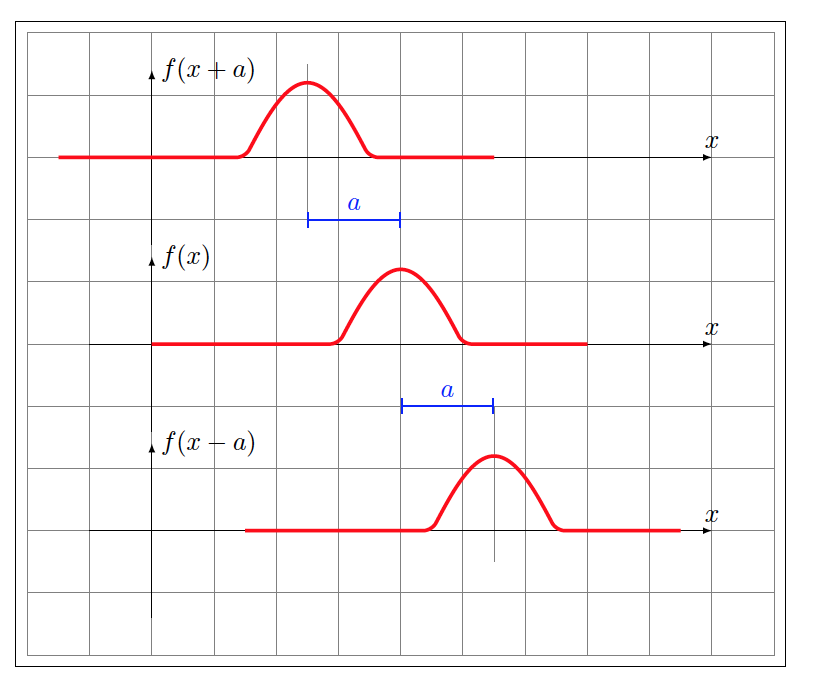
\includegraphics[width=160pt]{images/wellenrichtung.png}
\end{center}

\columnbreak


\subsection{Harmonische Wellen}
Laufende harmonische Welle:
\begin{equation*}
\xi(x,t) = \xi {_0} sin\lbrace k(x\pm vt) \rbrace
\end{equation*}

k = Wellenzahl $\> \>$ 
$\xi_0$ = Amplitude\newline
\newline

Wobei k und v:
\begin{equation*}
k(x+\lambda) = kx + 2\pi \> \Longrightarrow  \> k\lambda = 2\pi \> \Longrightarrow \> k = \frac{2\pi}{\lambda}
\end{equation*}
\begin{equation*}
v = \frac{\omega}{k} = \nu\lambda
\end{equation*}
\begin{equation*}
\nu = \frac{\omega}{\pi}
\end{equation*}
$\nu$ = Frequenz der Welle, $\omega$ = Kreisfrequenz,\newline v = Ausbreitungsgeschwindigkeit



\subsection{Ausbreitungsgeschwindigkeit der Welle}
Wellengleichung:
\begin{equation*}
\frac{d^2\xi}{dt^2} - v^2\frac{d^2\xi}{dx^2} = 0 
\end{equation*}
\newline
Einige Ausbreitungsgeschwindigkeiten:

\begin{center}
	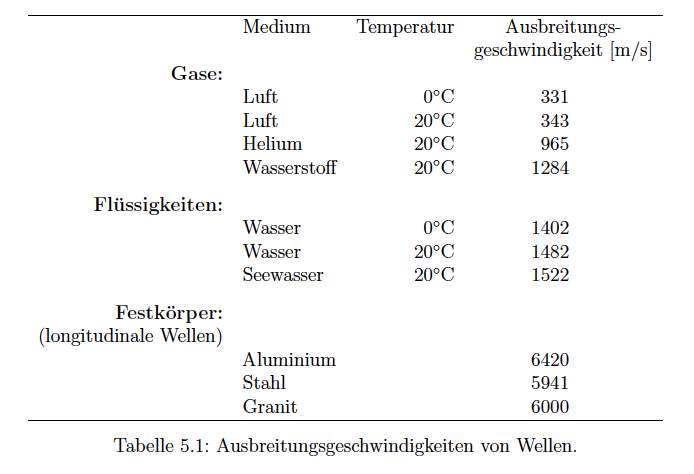
\includegraphics[width=250pt]{images/wellenausbreitungsgeschwindigkeit.png}
\end{center}

\columnbreak

\subsection{Ausbreitungsgeschwindigkeit transversaler, elastischer Seilwellen}
L{\"a}ngendichte des Seils:
\begin{equation*}
 p = \frac{M}{L}
\end{equation*}
M = Masse des Seils, L = L{\"a}nge des Seils\newline

\begin{equation*}
 v^2 = \frac{S}{p} \> \Longrightarrow \> v = \pm \sqrt{\frac{S}{p}}
\end{equation*}
wobei S die Spannung des Seils und p die L{\"a}ngendichte ist.
\newline 
 
\subsection{Wellen im Festk{\"o}rper}
Eine Deformation ist elastisch wenn der Festk{\"o}rper seine Form wieder annimmt, wenn die Kr{\"a}fte nicht mehr wirken.
\newline
Meisten K{\"o}rper sind nur bis zu einem bestimmten Grenze der Kr{\"a}fte elastisch = Elastizit{\"a}tsgrenze \newline
Relative L{\"a}ngen{\"a}nderung:
\begin{equation*}
\epsilon = \frac{\Delta l }{l}
\end{equation*}

Innerhalb der Elastizitätsgrenze gilt das Hooksche Gesetz:
\begin{equation*}
F = YA \frac{\Delta l}{l} = YA\epsilon
\end{equation*}
wobei: F = Kraft (die zieht), A = Querschnitt, Y = Elastizitätsmodul
\newline
\begin{center}
	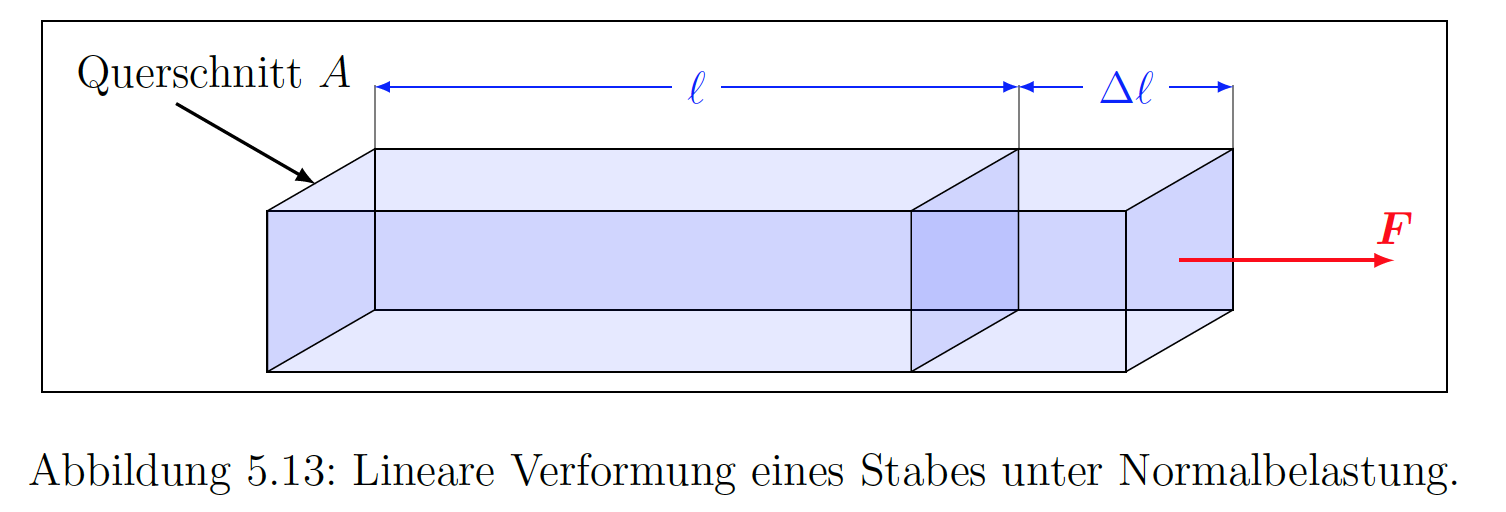
\includegraphics[width=250pt]{images/elastizitaetsmodul.png}
\end{center}

Einheit des Elastizit{\"a}tsmodul:
\begin{equation*}
\lbrack Y \rbrack = \frac{N}{m^2}
\end{equation*}

\paragraph{Deformationswellen}
\begin{enumerate}
  \item Longitudinale Wellen: Breiten sich in allen Medien aus.
  \item Transversale Wellen: Breiten sich nur in festen K{\"o}rpern aus
\end{enumerate}

\paragraph{Longitudinale, elastische Wellen im Festk{\"orper}}
\begin{equation*}
v^2 = \frac{Y}{P} \>\> \Longrightarrow \>\> v \pm \sqrt{\frac{Y}{p}}
\end{equation*}
Einheit des Elastizit{\"a}tsmodul ist wiederum:
\begin{equation*}
\lbrack Y \rbrack = \frac{N}{m^2}
\end{equation*}
\newline
Einige Ausbreitungsgeschwindigkeiten:
\begin{center}
	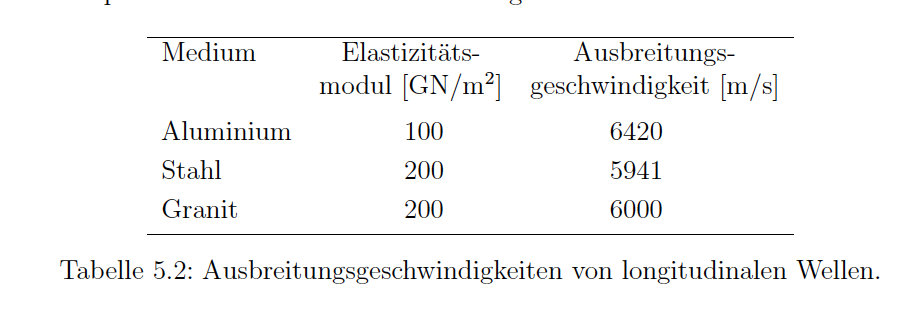
\includegraphics[width=250pt]{images/wellenausbreitungsgeschwindigkeit_long}
\end{center}

\subsection{Prinzip der Superposition}
Vereinfacht kann die Superposition folgendermassen ausgedr{\"u}ckt werden:
\begin{equation*}
\xi(x,t) = \xi _1(x-vt) + \xi _2(x+vt)
\end{equation*}
\newline
Sich aufsummierende Wellen:
\begin{center}
	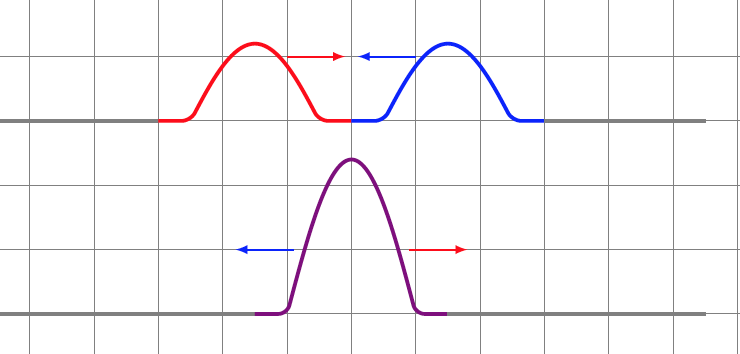
\includegraphics[width=180pt]{images/superposition2.png}
\end{center}
\columnbreak

Sich ausgleichende Wellen:
\begin{center}
	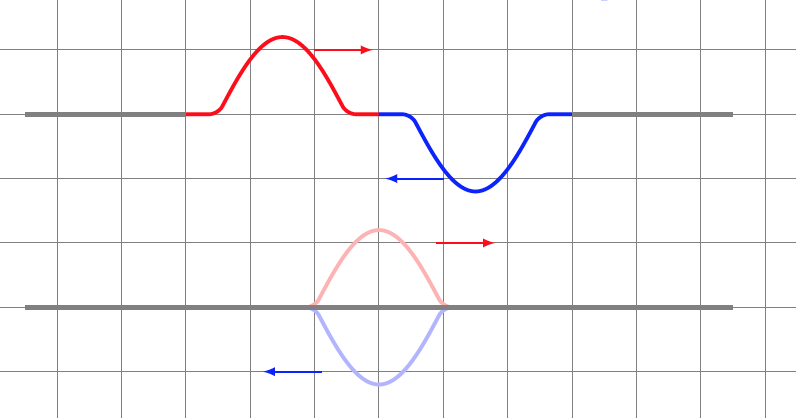
\includegraphics[width=180pt]{images/superposition1.png}
\end{center}

\subsection{Stehende Wellen}
Beispiel: Seite, die auf beiden Seiten befestigt ist. \newline
$\Longrightarrow$ Auslenkung in eine harmonische Schwingung durch eine {\"a}ussere Kraft\newline
\newline
Grundfrequenz = erste Eigenfrequenz $\nu_1$ $\Longrightarrow$ Die erste Welle davon = erste Harmonische \newline

Wellenl{\"a}nge:
\begin{equation*}
\lambda _n = \frac{2L}{n}
\end{equation*}
\newline
Eigenfrequenz $\nu_n$ :
\begin{equation*}
\nu _n = \frac{v}{\lambda _n} = n \frac{v}{2L}
\end{equation*}

wobei n = 1,2,3,... \newline

Die Frequenz der n'ten Harmonischen kann als Funktion der Grundfrequenz (erste Harmonische) betrachtet werden:
\begin{equation*}
\nu _n = n \nu _1
\end{equation*}
wobei:
\begin{equation*}
\nu _1 = \frac{v}{2L} 
\end{equation*}

Zudem folgt im Zusammenhang mit der bestimmten Geschwindigkeit:
\begin{equation*}
\nu _1 = \frac{1}{2L}  \sqrt{\frac{S}{p}}
\end{equation*}

\paragraph{Randbedingung stehender Wellen}\mbox{}\\
Aus dem Prinzip der Superposition folgt:

\begin{equation*}
\xi(x,t) = \xi _1(x,t) + \xi _2(x,t)
\end{equation*}
\begin{equation*}
= \xi _0 sin(kx-\omega t) + sin(kx+\omega t)
\end{equation*}
\begin{equation*}
= 2 \xi _0 sin(kx) + cos(\omega t)
\end{equation*}
\newline
Es folgt daraus, dass eine Punkt an einem beliebigen Ort x eine einfache harmonische Bewegung hat, und dass die Amplitude von Ort zu Ort verschieden ist.\newline
$\Longrightarrow$ Ist die Saite allerdings links und rechts befestigt, existiert eine Randbedingung bei x=0 (=L):
\begin{equation*}
\xi _0 (0,t) = \xi _0 (L,t) = 0
\end{equation*}

Daher folgt:
\begin{equation*}
\xi _0 (L,t) = 2 \xi _0 sin(kL) + cos(\omega t) = 0
\end{equation*}
\begin{equation*}
	\Longrightarrow sin(kL) = 0
\end{equation*}

\begin{center}
	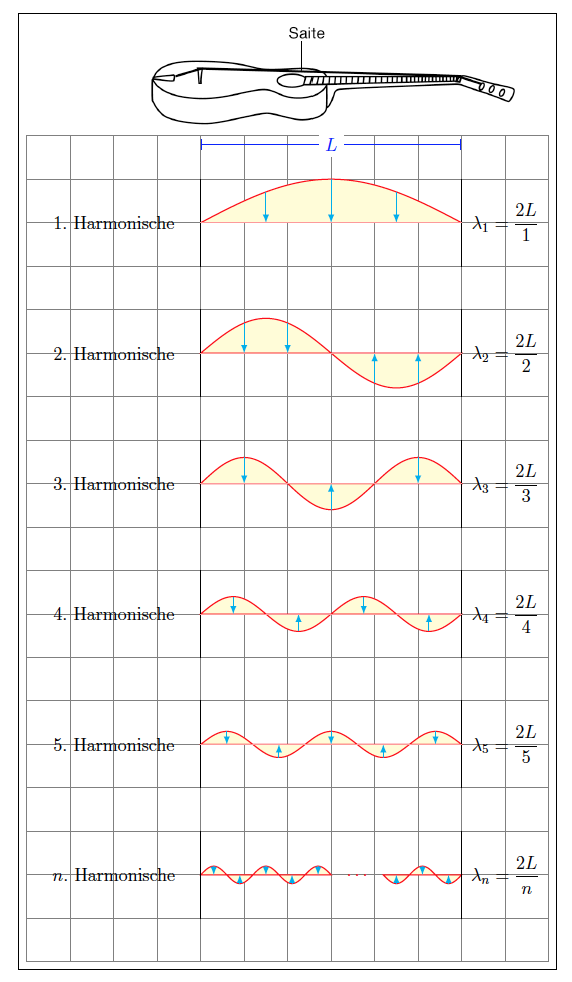
\includegraphics[width=150pt]{images/harmonische_saite.png}
\end{center}

\columnbreak

Die Bedingung wird erf{\"u}llt wenn die Wellenzahl k oder die Wellenl{\"a}nge folgende Werte besitzen:
\newline
\begin{equation*}
k_n L = \frac{2\pi}{\lambda _n}L = n\pi  \>\>\>\>\> n=1,2,3,...
\end{equation*}
oder:
\begin{equation*}
\lambda _n = \frac{2L}{n}  \>\>\>\>\> n=1,2,3,...
\end{equation*}


Wellenfunktion der n'ten Harmonischen:
\begin{equation*}
= 2 \xi _0 sin(k_n x) + cos(\omega _n t)
\end{equation*}

wobei:
\begin{equation*}
k_n = \frac{n\pi}{L} \>\> und \>\> \omega _n = 2\pi \nu _n \>\>\>\>\> n=1,2,3,...
\end{equation*}

\end{multicols*}
\end{document}